\documentclass[preprint,12pt]{elsarticle}
%\documentclass[review]{elsarticle}
\usepackage{lineno,hyperref}
\usepackage{booktabs}
\usepackage[english]{babel}
\usepackage[utf8]{inputenc}
\usepackage{amsfonts}
\usepackage{graphicx}
%\usepackage[colorinlistoftodos]{todonotes}
\usepackage{amssymb,amsmath}
\usepackage{float}
\usepackage{ragged2e}

\usepackage[utf8]{inputenc}
\usepackage{adjustbox}
\usepackage{multicol}
\usepackage{mwe}
%\usepackage{caption}
\usepackage[justification=centering]{caption}

\usepackage{algorithm}
%\usepackage{algorithm2e}
%\usepackage{algorithmicx}
\usepackage{algpseudocode}

\usepackage{multirow}
\usepackage{mathtools}  
\usepackage{graphicx}

\usepackage{color}
\usepackage{soul}
\usepackage{comment}

\usepackage{lscape}

\usepackage{setspace}
\doublespacing
%\linespread{1.5}


%\usepackage{caption,tabularx,booktabs}
\algnewcommand\algorithmicforeach{\textbf{for each}}
\algdef{S}[FOR]{ForEach}[1]{\algorithmicforeach\ #1\ \algorithmicdo}

\newcommand\tab[1][0.73cm]{\hspace*{#1}}

\usepackage{tikz}
\def\checkmark{\tikz\fill[scale=0.3](0,.35) -- (.25,0) -- (1,.7) -- (.25,.15) -- cycle;} 

\usepackage{array}
\newcolumntype{L}[1]{>{\raggedright\let\newline\\\arraybackslash\hspace{0pt}}m{#1}}
\newcolumntype{C}[1]{>{\centering\let\newline\\\arraybackslash\hspace{0pt}}m{#1}}
\newcolumntype{R}[1]{>{\raggedleft\let\newline\\\arraybackslash\hspace{0pt}}m{#1}}


\newcolumntype{P}[1]{>{\centering\arraybackslash}p{#1}}
\newcolumntype{M}[1]{>{\centering\arraybackslash}m{#1}}


%for vertical lines
\def\arrvline{\hfil\kern\arraycolsep\vline\kern-\arraycolsep\hfilneg}

\modulolinenumbers[5]

\journal{Elsevier}


%% `Elsevier LaTeX' style     
\bibliographystyle{elsarticle-num}
%%%%%%%%%%%%%%%%%%%%%%%


% Project tables and reproducible snapshot date; supplied template formatting is retained.
\usepackage{tabularx}
\hypersetup{hidelinks}
\def\today{October 11, 2026}

\usepackage{xurl}
\emergencystretch=2em
\begin{document}
\begin{frontmatter}
\title{WebSwipe: Mid-Air Word-Gesture Typing from a Single Uncalibrated Webcam}
\author[1]{Venkat Jaswanth (2023BCD0021)}
\author[1]{Shaun Alan Joseph (2023BCD0006)}
\author[1]{Akhil K (2023BCD0018)}
\author[1]{Nivien M. (2023BCS0054)}
\address[1]{Indian Institute of Information Technology, Kottayam, India}

\begin{abstract}
% Required: problem, issue, method, results and comparison metrics.
WebSwipe is an app that lets a user pinch / trace a word across an on-screen keyboard. It is designed to use only one RGB webcam. We fine-tuned a pretrained HaGRID YOLOv10n gesture detector alongside frozen MediaPipe tracking. To convert the swipes to words, we personalized a BiLSTM--CTC word decoder. On 29 webcam attempts, our pipeline increased complete capture from 8/29 to 23/29; decoder personalization increased correct first suggestions from 14/29 to 21/29. When we faced difficult lighting in recordings, our lighting adaptation recovered 15/15 swipes, with 11/15 correct first suggestions. We got trajectory degradation training to raise the top-1 accuracy from 74.6\% to 82.9\% across nine held-out-subject headset folds under simulated webcam degradation. This is versus 77.1\% for tuned SHARK2.

\end{abstract}
\begin{keyword}
Computer vision \sep Mid-air text entry \sep Hand gesture recognition \sep Transfer learning \sep BiLSTM \sep Connectionist temporal classification
\end{keyword}
\end{frontmatter}
\linenumbers

\section{Introduction}
% Required: domain introduction, explanatory figures, proposal, 2--3 contributions and organization.
Typing in the air is useful when a physical keyboard is out of reach or if we want a contactless interface, for example, when interacting with a display from a distance. Using a webcam, it is easy to observe the user's hand, but there are no physical keys to guide the movement. The system has to track the user's hand, identify when a gesture starts and ends, and convert the swipe into the intended word.

A word-gesture keyboard uses the path through a word's letters instead of one key at a time. SHARK2 used shape and location matching to compare such paths with a vocabulary \cite{shark2}. Shen et al. later introduced a learned trajectory decoder for augmented reality headsets \cite{shen2023}. We use these two ideas with a webcam, where hand tracking and pinch boundaries are less stable than the input they receive.

Recent text-entry studies examine recognition accuracy alongside typing speed, effort, and visual attention. The TEXT survey compares XR input methods and their evaluation protocols \cite{recent01}. Hu et al. studied the eye--hand coordination needed for mid-air typing \cite{recent02}. FineType uses a wrist-mounted infrared camera and inertial sensor for tapping-based input \cite{recent03}.

In WebSwipe, the right hand traces words and the left hand controls suggestions. A short left pinch cycles through the top 4 candidates; a held pinch deletes the word. Spaces are inserted automatically between words. The keyboard occupies about 45\% of the image width and sits toward the right. This is to reduce the movement needed to reach its keys. The app supports toggling the cursor, hand skeleton, and trail using C, H, and T, respectively. Hiding these overlays helps the user keep the mental model of swiping with the hand to type rather than moving the hand to move the cursor. Figure~\ref{fig:concept} illustrates the intended gesture.

\begin{figure}[H]
\centering
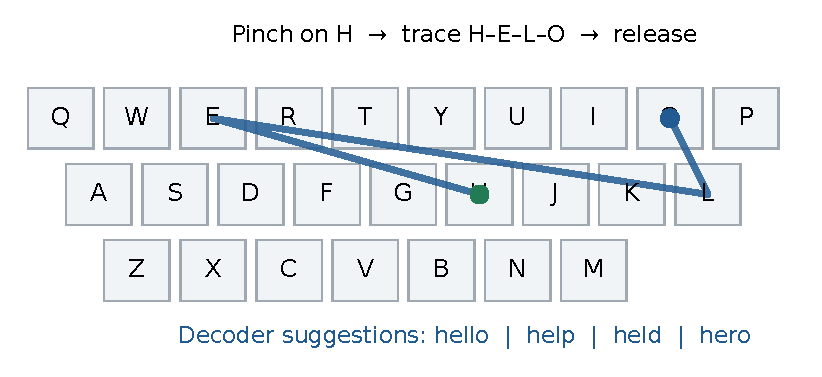
\includegraphics[width=\linewidth]{images/interaction.pdf}
\caption{WebSwipe interaction concept. The user pinches to start a gesture through the QWERTY layout and releases to decode the word. The path shown for ``hello'' is an illustration. Sequence decoding and vocabulary evidence resolve repeated letters.}
\label{fig:concept}
\end{figure}

Our main contributions are:
\begin{enumerate}
\item A working webcam word-gesture app. It combines hand tracking, pinch recognition, swipe segmentation, and word suggestions without having to calibrate the camera.
\item A PyTorch implementation of the Shen-style BiLSTM--CTC decoder. This was trained with trajectory degradation. It improves simulated-webcam top-1 accuracy by 8.3 percentage points over the clean model across nine held-out subjects.
\item Task-specific fine-tuning of the visual detector and personalization of the word decoder. This was supported by reusable recordings which let us reproduce failures, recover a difficult-lighting case, and separate missed swipes from incorrect word predictions.
\end{enumerate}

We developed the personalized system mainly with our own recordings. Our target was complete capture on at least 80\% of attempted words, using the span criterion defined in Section~\ref{sec:metrics}. Because we use only a single camera, we need to rely on the tracking and gesture recognition to handle different depths, viewpoints and lighting effects.

Section 2 reviews related work. Section 3 explains the app and its training stages. Section 4 presents the datasets, results, and failure analysis. Section 5 summarizes what we achieved and the remaining work.

\section{Related works}\label{section2}
% Required: at least 15 articles after 2024, their problems/methods/results,
% four or five relevant limitations, and the scope addressed here.
SHARK2 compares a gesture with ideal word paths using shape and location matching \cite{shark2}. We use it as a template baseline. Shen et al. use a learned trajectory decoder for mid-air headset input \cite{shen2023}. Their released model and data form the basis of our neural decoder. We keep the same sequence representation and adapt training and input capture to a webcam. We also discuss 15 studies from 2025. These cover the sensing setup, hand tracking and gesture recognition, and ways to handle imperfect camera input.

\subsection{Text entry without surface contact}
The TEXT trove organizes XR text-entry techniques by sensing and interaction method \cite{recent01}. The sensing setup and interaction methods help explain the differences between reported typing speeds. For example, FineType combines an infrared camera and an IMU in a wristband to recognize finger combinations and tapping postures with a multi-task convolutional network \cite{recent03}. It reports 94.19\% cross-user gesture accuracy. After only two hours of practice, users reach 35.1 words per minute with a 5.1\% character error rate. The problem is that it depends on a wearable sensor and surface contact.

Hu et al. compared tablet and mid-air gesture typing with 16 participants \cite{recent02}. They found that expert users could reach comparable text-input performance. Mid-air input needed more attention to the keyboard and closer eye--hand synchronization. This shows why visual feedback matters for the interaction. In WebSwipe, the keyboard and gesture-state feedback stay visible, while the user can hide the cursor and trail.

\subsection{Hand position and 3D reconstruction}
For word input, we need a stable hand position in the keyboard plane. WiLoR combines real-time hand localization with transformer-based reconstruction \cite{recent04}. It introduces over two million hand images with different appearances, lighting conditions, and occlusions, and improves efficiency and accuracy on hand benchmarks. HandOS predicts detection, 2D joints, and 3D reconstruction together to reduce errors between separate stages \cite{recent11}. Its interactive decoder and hierarchical attention achieve a PA-MPJPE of 5.0 on FreiHand and 64.6\% PCK at a 0.05 threshold on HInt-Ego4D. We use a separate tracker and small gesture detector so we can inspect the position and pinch decisions. Tracking errors can still affect the word decoder.

HOT3D, Dyn-HaMR, and UniHOPE address more complex scenes. HOT3D provides multi-view hand--object data and shows improved tracking with multiple views \cite{recent05}. Dyn-HaMR combines SLAM and hand-motion priors to improve reconstruction when the camera moves or the hand is occluded \cite{recent06}. UniHOPE uses grasp-aware fusion and de-occluded training to improve estimation on bare-hand and hand--object benchmarks \cite{recent07}. WebSwipe maps movement in the image plane, so occlusion and viewpoint changes remain problems for our setup.

\subsection{Keeping motion stable and recognizing contact}
Missing hand observations can break a swipe. HaWoR uses camera-motion estimation and fills gaps in motion to improve world-space hand tracking \cite{recent09}. Fan et al. combine temporal joints and image features for competitive low-resolution reconstruction on three benchmarks \cite{recent12}. Liu et al. combine visual, joint, and direction features with confidence estimates to reduce jitter \cite{recent15}. They report improved results on FreiHand and HO3D. We use temporal filtering and allow short tracking gaps to keep the recorded path stable.

Tracking the hand also leaves the problem of deciding whether the fingers are touching. EgoPressure provides pressure and pose annotations, and its models find useful complementary information in both signals \cite{recent10}. Fingertips can look close in the image without touching. We therefore combine appearance, geometry, and motion for the left-hand controls. GigaHands uses markerless capture to provide 34 hours of two-hand activity from 56 participants \cite{recent08}. The data supports motion synthesis and captioning. Our recordings focus on typing and its controls.

\subsection{Training for the input the camera actually sees}
FoundHand uses a diffusion model conditioned on keypoints and masks to generate hand images with controlled poses and appearance transfer \cite{recent13}. Zhao et al. study how forearm context, image statistics, pose, and occlusion affect synthetic-to-real transfer \cite{recent14}. Combining these factors matches real-data pose accuracy in their tested setting. Our coordinate degradation handles a narrower part of the input mismatch. We use real camera recordings to adapt the visual detector.

\subsection{Limits that shaped our evaluation}
We had four main challenges: using a single front-facing camera, keeping a complete word path when tracking is interrupted, adapting to different hands and lighting, and measuring typing speed and effort along with recognition accuracy.

Our main focus is the camera pipeline and capturing complete swipes. We use fine-tuning to adapt the models to the input. Reusable recordings let us check whether a failure came from capturing the swipe or ranking the intended word.

\section{Proposed Method}
% Required: proposal introduction, architecture diagram and explanation, algorithm and explanation.
We handle hand position and gesture recognition separately. MediaPipe provides the landmarks used for the cursor and hand crops. Two fine-tuned gesture models provide pinch and release evidence. A state machine selects the points that belong to the swipe, and a neural decoder ranks the words. This lets us check where a failure happened. We started with Kinivi's MediaPipe gesture-recognition example and added the keyboard, recording tools, word decoder, and interaction logic \cite{kinivi}.

\subsection{Architecture and image-plane coordinates}
\begin{figure}[H]
\centering
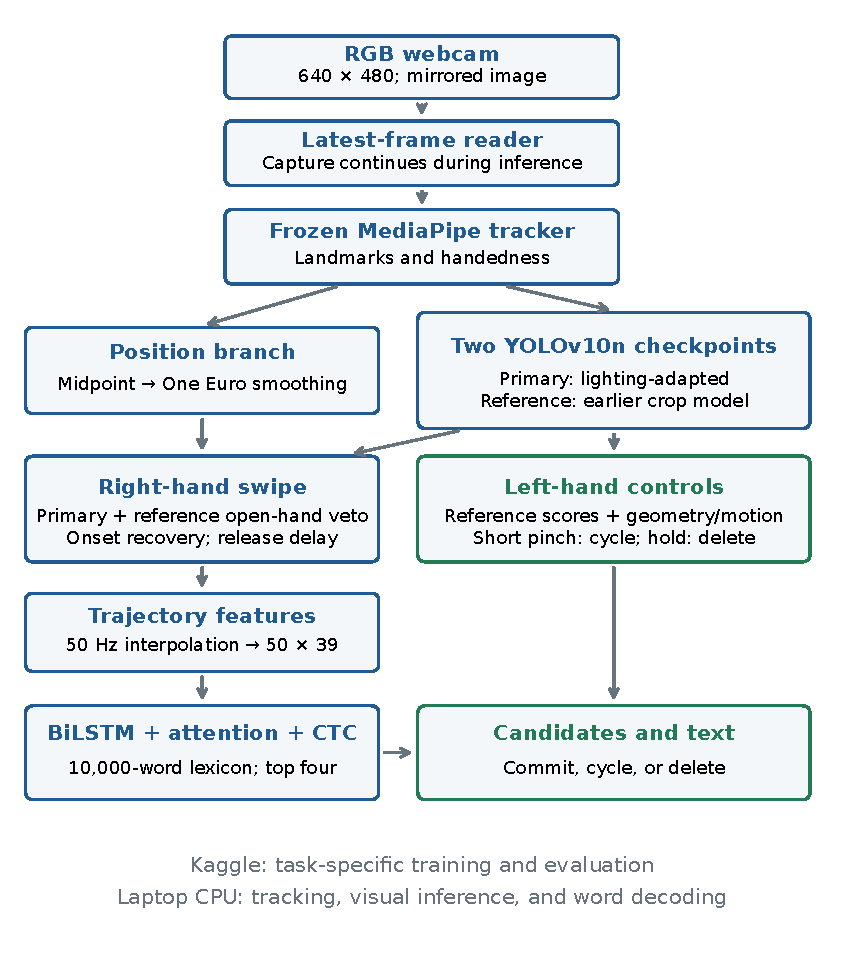
\includegraphics[width=\linewidth]{images/architecture.pdf}
\caption{WebSwipe data flow. The frozen hand tracker provides coordinates and hand crops. The lighting-adapted detector provides the main pinch scores. The earlier crop detector can reject a right-hand pinch and provides appearance scores for the left hand. Both hands control the same displayed text. Training runs on Kaggle, while the app runs inference on the laptop CPU.}
\label{fig:architecture}
\end{figure}

The app mirrors the camera image and corrects the handedness labels. This keeps the physical hands assigned to their intended roles. MediaPipe Hand Landmarker returns 21 landmarks for each hand \cite{mediapipe,mediapipehands}. We keep its weights frozen. A background camera reader keeps the newest frame ready for processing. This prevents old frames from building up in a queue. Capture and processing run at different rates, and each processed observation keeps its timestamp.

Let $\mathbf{l}_{4,t}$ and $\mathbf{l}_{8,t}$ denote the thumb-tip and index-tip pixel positions. The cursor is their midpoint,
\begin{equation}
\mathbf{c}_t=\frac{\mathbf{l}_{4,t}+\mathbf{l}_{8,t}}{2}.
\end{equation}
We use a One Euro filter to smooth the cursor based on the observed frame interval \cite{oneeuro}. Its cutoff increases when the hand moves faster. This reduces jitter at rest while allowing faster movement. The app then converts the filtered image point to keyboard coordinates by subtracting the overlay origin and reversing the vertical axis:
\begin{equation}
\mathbf{q}_t=(c_{x,t}-x_0,\;-(c_{y,t}-y_0)).
\end{equation}
This conversion puts the swipe coordinates in the keyboard's image-plane coordinate system. The user follows the on-screen keyboard, which occupies about 45\% of the image width. The window starts at 1280 by 960 pixels and can be resized.

\subsection{Hand-crop gesture recognition and swipe boundaries}\label{sec:pinch}
We start with the released HaGRID YOLOv10n gesture checkpoint, \nolinkurl{YOLOv10n_gestures.pt}. We fine-tune it on our gesture data \cite{yolov10,hagridv2}. There are four class names: \texttt{ok}, \texttt{palm}, \texttt{fist}, and \texttt{no\_gesture}. The \texttt{ok} class provides pinch evidence. We also include open palms and other non-pinching poses as negative examples. These include fingers held close together without touching. Training starts from the pretrained gesture weights, followed by webcam adaptation, hand-crop adaptation, and lighting adaptation. We export the selected checkpoints to ONNX to run inference on the CPU.

The crop is centered on the landmark bounding box. We add a 12\% margin on each side and expand the largest dimension by 1.35 to make a nominal square crop. The crop is clipped to the frame. If either dimension is smaller than 20 pixels, it is rejected. Before inference, the crop is resized and padded to $320\times320$ pixels. BGR is converted to RGB, and intensities are scaled to $[0,1]$. The predicted boxes are converted back to frame coordinates. A box is assigned to a tracked hand when its intersection-over-union with the hand box is at least 0.3.

The final app runs both selected detectors on each tracked hand crop. For the right hand, the lighting-adapted detector provides the main scores. If the earlier crop detector gives \texttt{palm} or \texttt{no\_gesture} a score of at least 0.5, the app sets the main pinch score to zero. The reference detector can reject a pinch, but it cannot start one. For the left hand, we use the earlier crop detector's scores directly.

After the reference check, the dominant-hand setup uses score hysteresis. A pinch starts when at least two of the last three observations reach 0.5, and an ongoing pinch continues while its score remains above 0.3. The word segmenter waits for 80 ms of release evidence before it commits. Points observed after the pinch switches off are not included in the word path. A missing-hand interval may be bridged for up to 200 ms. Any longer than that, and it ends the segment. To decode a gesture, we need at least 4 points.

A late pinch decision can miss the first letter of a swipe. We use an evidence-filtered onset buffer to recover up to 700 ms of preceding continuous movement. It includes contact-like points, or near-contact points with supporting appearance evidence. It excludes ordinary hovering. This recovery does not join separately completed gestures. Merged attempts still count as evaluation failures.

The geometric evidence uses a scale-normalized pinch ratio,
\begin{equation}
r_t=\frac{\lVert\mathbf{l}_{4,t}-\mathbf{l}_{8,t}\rVert_2}
{\widehat{\lVert\mathbf{l}_{0,t}-\mathbf{l}_{9,t}\rVert_2}},
\end{equation}
The denominator is a running estimate of palm length. The contact rule uses the median normalized gap over three observations. Contact turns on below 0.20 and turns off at 0.27. The right-hand pinch state uses appearance scores. The geometric evidence also helps recover the start of its swipe.

The left-hand controls combine the geometric contact rule with appearance evidence. The app can also recognize a brief pinch from consecutive observations of the fingertips closing, before the median contact filter responds. Recent opening and closing motion helps separate a pinch from fingers resting close together. Geometric and visual release checks end the pinch. A short re-entry guard reduces duplicate commands. The \hyperref[app:reproducibility]{reproducibility appendix} lists the thresholds and timing windows.

\subsection{Trajectory features and neural word decoding}
Our neural decoder is a PyTorch implementation of the released Shen-style architecture \cite{shen2023,shencode}. We first interpolate the timestamped coordinates onto a uniform 50 Hz clock. This keeps the seven-sample, third-order Savitzky--Golay smoothing window consistent across different input rates \cite{savitzkygolay}. We then resample the smoothed path to 50 points for the sequence model.

Each point has 39 features. These include two coordinates normalized by the keyboard dimensions, 26 key-proximity indicators, and 11 local path descriptors. The descriptors represent displacement, curvature, local aspect ratio, slope, path curling, and linearity. We keep the repeated displacement entries from the released feature representation. Before inference, we replace non-finite values and clip extreme values.

The model has two bidirectional LSTM layers. Each has 400 hidden units per direction, with input dropout of 0.2. After the second layer, the forward outputs provide queries $Q$. The backward outputs provide keys and values $V$. Attention and output logits are computed as follows:
\begin{equation}
A=\operatorname{softmax}(QV^\top),\qquad Z=(AV)W_o+b_o.
\end{equation}
Our output contains 29 classes: 26 letters, a word-boundary token, a CTC blank, and one additional index retained for compatibility. Our training uses CTC loss \cite{ctc}, which sums over admissible alignments between steps and the target character sequence.

The vocabulary decoder uses a dynamic program to compute a CTC score for each word. It ranks the words in a fixed lexicon and returns four suggestions. It can only suggest words from that lexicon. The live demo uses 10,000 words. Our experiments on D1, the recorded headset-typing dataset released by Shen et al., use its closed vocabulary of 1,996 words.

For a candidate word $w$, the live score is
\begin{equation}
s(w)=\log P_{\mathrm{CTC}}(w\mid Z)-\gamma E(w)+\lambda\log p(w),
\end{equation}
where $E(w)$ penalizes disagreement between the recorded endpoints and the first and last letter centers:
\begin{equation}
E(w)=\min\left(12,\frac{\lVert\mathbf{q}_{\rm start}-\mathbf{k}_{w_1}\rVert^2+
\lVert\mathbf{q}_{\rm end}-\mathbf{k}_{w_{|w|}}\rVert^2}{2p^2}\right).
\end{equation}
Here $p$ is key pitch. Our installed setup uses $\gamma=1$ and $\lambda=0$. The decoder supports a unigram prior, but this did not improve the evaluated neural decoder enough for us to use it. It does improve the SHARK2 baseline's ranking of common words.

\subsection{Training and task-specific fine-tuning}
We first train the word decoder on the recorded headset trajectories using our PyTorch implementation of the released architecture. Each leave-one-subject-out fold has two models: a clean model and an augmented model. Both use the same architecture, RMSprop, a learning rate of $10^{-4}$, and a batch size of 64. The reported LOSO models are trained for 100 epochs, and we use the final checkpoint. We do not use the held-out subject to pick the best epoch. There is one training seed per fold.

For augmented training, we apply randomized degradation to 50\% of gestures and compute their features again. The frame rate is chosen from native, 30, 20, 15, 12, and 10 fps. Gaussian jitter ranges from 0 to 0.3 key widths. The end-truncation limit is chosen from 0, 50, or 100 ms. These changes simulate errors in coordinate sampling and gesture boundaries.

We first fine-tuned the released gesture checkpoint on labeled webcam images. This detector and the older examples were the starting point for crop adaptation. The crop continuation uses 183 newly reviewed training frames, 46 new development frames, 1,595 older training examples, and 700 HaGRID replay examples. We repeat new pinch examples three times and new negative examples ten times to give them more weight. After cropping and repetition, there are 3,347 training entries and 457 validation crops. Repetition changes how often an image is used, without adding independent images. Training uses AdamW with a learning rate of $3\times10^{-4}$, a batch size of 32, and up to 15 epochs. We use seed 42 and $320\times320$ input. Augmentation includes modest rotation and scale changes, with no mosaic or mixup. We export the checkpoint with the best validation result. The hand tracker stays frozen throughout.

For lighting adaptation, we continue from the selected crop checkpoint. We add 85 reviewed training frames and 90 development frames. With the earlier crop data, this gives 268 reviewed training frames and 136 development frames. We also retain the 1,595 older training examples and 700 HaGRID replay examples. Weighting and cropping give 3,937 training entries and 547 validation crops. We train with AdamW for 8 epochs, using a learning rate of $10^{-4}$, a batch size of 32, seed 42, and $320\times320$ input. The earlier crop checkpoint stays in the app as the reference model. MediaPipe stays frozen during both stages.

We personalize the word decoder with 79 reviewed air-swipe traces. These include 41 recovered early-session gestures and 38 older accepted guided traces. We use RMSprop with a learning rate of $10^{-5}$ for ten epochs, a batch size of 32, and gradient clipping at 5. Each epoch includes four versions of the air traces and 512 D1 replay examples from subjects other than subject 0. Three versions use small scale and translation changes. Development evaluation has 45 intended attempts, but only 44 captured trajectories. The missing attempt still counts as a failure. We also check five older traces and a fixed 512-example D1 sample from subject 0. We compare epochs 2, 5, and 10 against predefined improvement and non-regression conditions and select epoch 10. This adapts the decoder to the recorded user.

\subsection{End-to-end algorithm and bimanual controls}
\begin{algorithm}[H]
\caption{WebSwipe inference for each timestamped camera frame}
\label{alg:webswipe}
\begin{algorithmic}[1]
\Require RGB frames, frozen tracker, primary and reference gesture detectors, word decoder, keyboard geometry, lexicon
\Ensure Committed words and up to four suggestions per released gesture
\State Initialize cursor filter, pinch filters, swipe segmenter, and control state
\ForEach{newest available frame $I_t$ with timestamp $t$}
\State Mirror $I_t$; estimate landmarks and correct physical handedness
\State Crop hands; infer and assign scores from both gesture detectors
\State Veto right-hand pinch when the reference predicts an open hand
\State Filter the dominant-hand midpoint and map it to keyboard coordinates
\State Update pinch hysteresis and evidence-filtered onset lookback
\State Update the swipe segmenter using pinch state, tracking gaps, and release delay
\If{a completed trajectory with at least four points is returned}
\State Resample at 50 Hz, smooth, and extract $50\times39$ features
\State Compute BiLSTM--attention logits and lexicon CTC scores
\State Apply endpoint penalty; return the four highest-scoring words
\State Commit the first suggestion and update displayed text
\EndIf
\State Fuse left-hand reference scores, fingertip geometry, and recent motion
\State Brief control pinch cycles suggestions; a 0.6 s hold deletes the last word
\State Render keyboard, status feedback, text, and enabled overlays
\EndFor
\end{algorithmic}
\end{algorithm}

Algorithm~\ref{alg:webswipe} runs continuously. The pinch state decides which points belong to a swipe. Decoding starts after release. A short left pinch cycles through the last word's candidates, while a 0.6-second hold deletes the word once. Keys 1--4 select a candidate, and B deletes. Normal demo logs save word candidates, event times, point counts, decoder timing, and control actions. The dedicated recording modes also save full swipe paths and camera video.

\subsection{Recording and failure diagnosis}
Swipes sometimes broke before the word was finished, and the final suggestion did not show where the failure happened. We built a recorder to save the camera frames, hand landmarks, intended word, and captured path. Space-key markers record the intended swipe interval. Replaying these recordings let us separate incomplete capture from incorrect word predictions and compare fixes on the same attempts.

We also built a prompted pinch recorder to investigate unreliable left-hand controls. It saves the hand video and the app's decisions, then shows whether each attempt triggered a cycle or delete. This let us compare visible pinches with missed or unintended commands and adjust the control rules using the recorded evidence.

\begin{figure}[H]
\centering
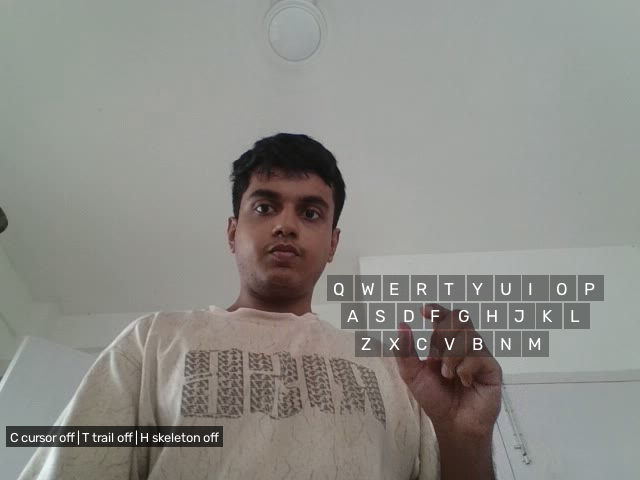
\includegraphics[width=.82\linewidth]{images/app_replay_standing.png}

\smallskip
\begin{minipage}[t]{.48\linewidth}
\centering\small Candidates and pinch state\par\smallskip
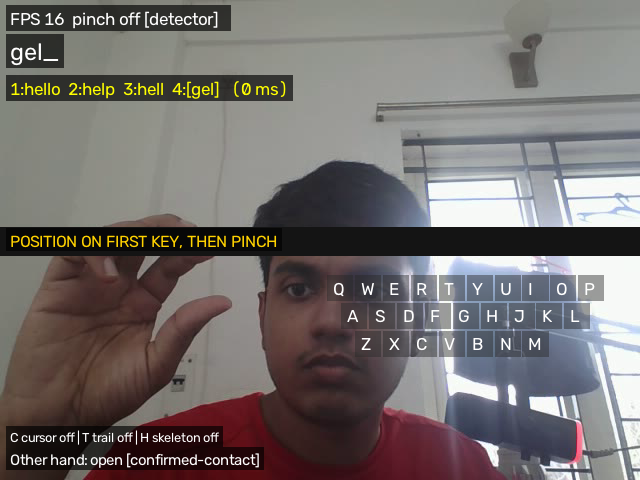
\includegraphics[width=\linewidth,viewport=0 375 300 480,clip]{images/app_replay.png}
\end{minipage}\hfill
\begin{minipage}[t]{.48\linewidth}
\centering\small Keyboard detail\par\smallskip
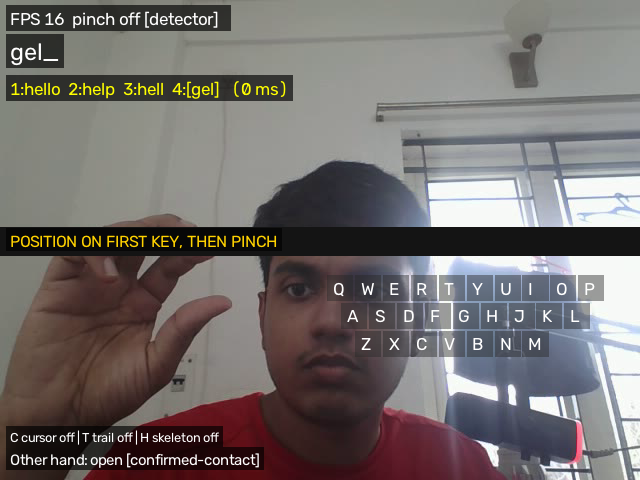
\includegraphics[width=\linewidth,viewport=320 118 610 210,clip]{images/app_replay.png}
\end{minipage}
\caption{The app's keyboard overlaid on a saved standing frame, with candidate and keyboard details from the earlier interface replay below. The cursor, trail, and skeleton are hidden. The recorded-frame interface replay uses preloaded candidates; its timing field is a placeholder.}

\label{fig:app}
\end{figure}



\section{Datasets and Experimental results analysis}
% Required: datasets and table, setup, explained tables/graphs/case studies, final performance comparison table.
We use three types of evaluation. The nine-subject D1 experiment tests the decoder on held-out headset trajectories with simulated degradation. The webcam replays test the full pipeline on recordings reused during development. Synthetic paths let us examine individual noise and preprocessing effects. The webcam results cover missed swipes, improvements in word ranking, and the later lighting failure and recovery.

\subsection{Datasets and partitions}
\begin{table}[!htbp]
\centering
\caption{Data actually used and its role. Counts refer to filtered records and saved adaptation inputs.}
\label{tab:data}
\begingroup\small\setstretch{1.15}
\begin{tabularx}{\linewidth}{>{\raggedright\arraybackslash}p{2.8cm}>{\raggedright\arraybackslash}p{3.3cm}>{\raggedright\arraybackslash}X}
\toprule
Data & Available count & Role and partition \\
\midrule
D1: Shen headset traces & 18,055 filtered gestures; 1,996 words; 9 subjects & Decoder training and nine LOSO tests; original recorded data, with optional simulated degradation \\
Synthetic QWERTY traces & 3,000-word lexicon in the initial experiments & Noise, normalization, filtering, and decoder analyses; ideal generated paths \\
Gesture crop adaptation & 183 reviewed training frames; 46 development frames & Earlier crop stage; combined with 1,595 older examples and 700 HaGRID replay examples \\
Lighting continuation & 85 added training frames; 90 added development frames & Totals: 268 reviewed training and 136 development frames; same older-data replay pool \\
Air-swipe personalization & 79 training traces; 45 intended development attempts; 5 supplementary traces & Single-user decoder adaptation; 44 development traces actually captured \\
Original webcam check & 29 attempts: 15 sitting, 14 standing & Originally reserved chronological block; later reused for regression checks \\
Difficult-lighting check & 15 standing attempts & Earlier lighting failure and later recovery; reused during development and kept separate from the original 29 \\
\bottomrule
\end{tabularx}
\endgroup
\end{table}

Separate control recordings cover non-pinching hand movement and prompted brief or held pinches. These let us compare the intended actions with the commands registered by the app.

D1 comes from the released headset dataset \cite{shen2023,shencode}. Our preprocessing keeps alphabetic word gestures with at least four points. The phrase and suggestion lists must have matching lengths, and the intended word must appear in the original suggestion list. This gives a tensor of shape $18{,}055\times50\times39$. The nine subject identifiers are 0, 1, 2, 4, 5, 6, 7, 8, and 9. The reported D1 accuracy uses this filtered dataset and its closed vocabulary.

The gesture detector uses a HaGRID subset and our labeled examples. HaGRIDv2 discusses how varied negative hand movements help reduce false positives \cite{hagridv2}. We use the subset and replay counts listed above. We review labels from sampled video intervals and generate the boxes from landmarks. Adjacent frames and repeated crops are correlated examples.

For crop adaptation, we used training frames from the first 90 seconds of the reviewed sessions and development frames from before 180 seconds. We initially kept the later word blocks, around 180/185--240 seconds, separate. We chose the crop configuration using the development data before checking those later blocks. We then reused the recordings during personalization and lighting work. The final webcam results show our progress on those same sessions. Teammate data was excluded from the selected training and model selection.

\subsection{Experimental setup and metrics}\label{sec:metrics}
The app runs on a Linux laptop with an AMD Ryzen 7 7730U, eight physical cores, 16 logical processors, and about 13 GiB of usable memory. Training ran on Kaggle GPUs. The app uses Python 3.13, OpenCV, MediaPipe Tasks, PyTorch, NumPy/SciPy, and ONNX Runtime. Capture targets $640\times480$ images at a nominal 30 fps. During the recorded pinch diagnostic, capture ran at 29.6 fps and processing at 16.0 fps. These are session throughput measurements, including recording overhead.

The selected app uses the lighting-adapted detector, the earlier crop detector as a reference, the personalized word decoder, and the frozen MediaPipe tracker. The \hyperref[app:reproducibility]{reproducibility appendix} lists the exact filenames, model hashes, software versions, and evidence locations.

The D1 tests train on eight participants and test on the remaining one. All decoders receive the same degraded trajectories and use 50 Hz preprocessing. The simulated webcam preset uses 12 fps, 0.15 key-width Gaussian jitter, and up to 100 ms of truncation at each end. The harsh preset uses 10 fps, 0.3 key-width jitter, and the same truncation. We report the unweighted mean and sample standard deviation across subjects. Each subject contributes equally, regardless of how many retained words they have.

For webcam replay, complete capture means one finished, unmerged segment covering at least 80\% of a Space-marked intention interval. The Space markers define when the user intends to start and end the word. A segment needs at least four points. Missed, split, merged, and unfinished attempts still count in the denominator. Top-1 means the intended word is the first suggestion. Top-4 means it appears among the first four suggestions:
\begin{equation}
\mathrm{Acc@}k=\frac{\text{intended attempts with the target in the first }k\text{ candidates}}
{\text{all intended attempts}}.
\end{equation}
Capture and word correctness measure different things. The 80\% span rule applies to each attempted swipe. A short but completed trace can sometimes predict the right word even when it does not meet that capture rule.

\textbf{Evaluation scope.} We developed and checked the webcam setup using one user's recordings. We reused these sessions while choosing models and control rules. Testing with new users is the next step. A controlled typing study is still needed to measure words per minute, character error rate, and end-to-end latency. Webcam pinch F1 would also need labels showing when the fingers physically touched. The pinch-F1 and template-runtime results in the supporting notes come from simulations.

\subsection{Decoder robustness on D1}
\begin{table}[H]
\centering
\caption{Local decoder comparison on matched D1 LOSO tests: top-1 accuracy (\%), mean $\pm$ standard deviation across nine subjects. Both SHARK2 variants use smoothing and 50 Hz preprocessing. The tuned-prior variant was evaluated on clean and webcam conditions only.}
\label{tab:loso}\label{tab:comparison}
\begingroup\footnotesize\setstretch{1.15}
\setlength{\tabcolsep}{3pt}
\begin{tabularx}{\linewidth}{@{}Xrrrr@{}}
\toprule
Condition & \shortstack{SHARK2\\no prior} & \shortstack{SHARK2\\tuned prior} & \shortstack{Clean\\BiLSTM} & \shortstack{Augmented\\BiLSTM} \\
\midrule
Clean & $67.8\pm20.3$ & $77.5\pm21.2$ & $86.3\pm12.9$ & $86.6\pm15.9$ \\
30 fps & $70.3\pm21.3$ & --- & $85.8\pm12.6$ & $86.5\pm15.8$ \\
12 fps & $71.6\pm21.6$ & --- & $82.8\pm13.4$ & $85.4\pm15.4$ \\
Jitter 0.1 & $66.6\pm20.0$ & --- & $86.5\pm13.0$ & $86.9\pm15.7$ \\
Jitter 0.2 & $63.1\pm18.5$ & --- & $86.3\pm12.8$ & $86.8\pm15.7$ \\
Jitter 0.3 & $58.1\pm16.3$ & --- & $85.5\pm13.0$ & $86.4\pm15.0$ \\
Webcam preset & $69.0\pm9.1$ & $77.1\pm7.4$ & $74.6\pm12.5$ & $82.9\pm10.0$ \\
Harsh preset & $61.3\pm7.8$ & --- & $69.3\pm13.4$ & $78.5\pm11.3$ \\
\bottomrule
\end{tabularx}
\endgroup

\end{table}

On clean data, the clean and augmented models differ by 0.3 percentage points. Under the webcam preset, augmentation improves accuracy by 8.3 points. Under the harsh preset, the gain is 9.2 points. The augmented model beats the clean model in every held-out fold under these two presets.

\begin{figure}[H]
\centering
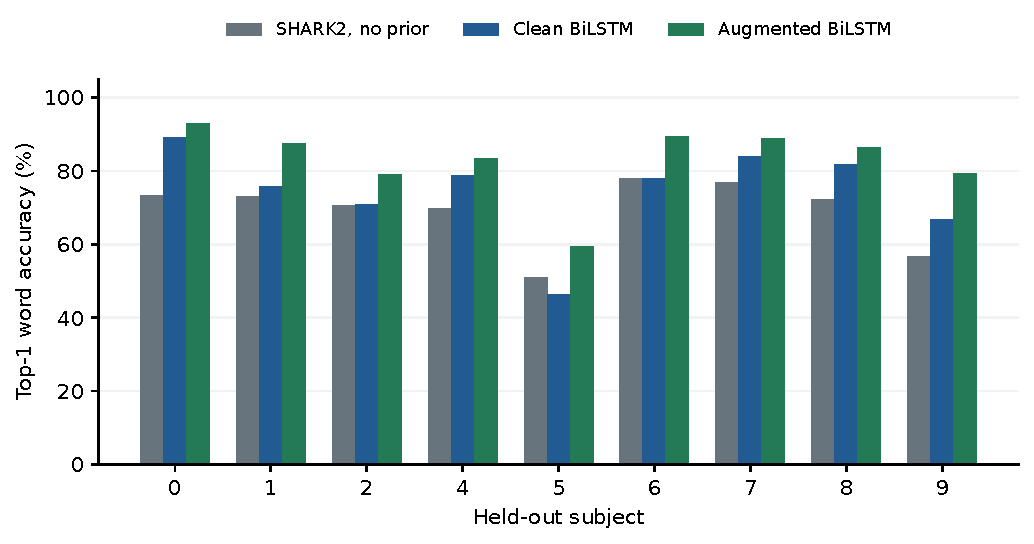
\includegraphics[width=\linewidth]{images/loso.pdf}
\caption{Per-subject top-1 accuracy under the simulated webcam preset on D1. Each subject is excluded from neural training; trajectories are already recorded and segmented. SHARK2 in this figure has no word-frequency prior.}
\label{fig:loso}
\end{figure}

Figure~\ref{fig:loso} shows differences between users. Subject 9's results change substantially with timestamp-based preprocessing. Its augmented-model accuracy is 44.8\% on clean input after 50 Hz preprocessing, compared with 86.0\% without that step and 79.4\% under the webcam preset. We keep this subject in the results along with the other eight.

SHARK2 also scores higher at lower frame rates. Interpolation changes the path before smoothing and matching. Under the webcam preset, subject 9 improves from 13.8\% to 56.7\%, while the other eight subjects' mean falls. Their scores become closer, so the spread decreases. Both interpolation and endpoint truncation change the input here, and we have not measured their effects separately.

The strongest SHARK2 baseline uses a word-frequency prior tuned on the other participants. It reaches 77.1\% under the webcam preset. The augmented decoder exceeds this by 5.8 points.

\subsection{Webcam capture and personalization results}
\begin{table}[H]
\centering
\caption{Replay of the same 29 webcam attempts. All percentages use 29 attempts, including failures. Configurations with identical counts share a row.}
\label{tab:webcam}
\begingroup\small\setstretch{1.15}
\begin{tabularx}{\linewidth}{Xccc}
\toprule
Configuration & Complete capture & Correct top-1 & Correct top-4 \\
\midrule
Initial / continued detector + original decoder & 8 (27.6\%) & 5 (17.2\%) & 6 (20.7\%) \\
Crop detector + original decoder & 23 (79.3\%) & 14 (48.3\%) & 18 (62.1\%) \\
Personalized decoder with crop detector / selected lighting + reference setup & 23 (79.3\%) & 21 (72.4\%) & 22 (75.9\%) \\
\bottomrule
\end{tabularx}
\endgroup
\end{table}

The recordings showed that the app often failed to retain a complete swipe. With hand-crop detection and the updated pinch and segmentation logic, complete captures increased from 8/29 to 23/29, a gain of 51.7 percentage points. Keeping these recordings fixed then let us evaluate word-decoder personalization separately.

Keeping the fixed crop pipeline, personalization raises first-suggestion accuracy from 14/29 to 21/29, which is a 24.1-point gain. Capture remains 23/29 because the word-model updates do not change the segmentation branch. Personalization improves ranking only within the captured traces. The installed configuration achieves our original 80\% capture target.



% P095: Detailed cadence replays are retained in evidence/diagnostic_detail_notes.tex.

The lighting update keeps capture at 44/45 on the older development attempts. Compared with the personalized crop setup, top-1 falls from 39/45 to 38/45 and top-4 from 44/45 to 42/45. This was the trade-off for recovering the difficult-lighting recording while retaining the original 29-attempt results.

\subsection{Case studies: posture, lighting, and control errors}
\begin{table}[H]
\centering
\caption{Capture and top-1 counts for each condition, shown as earliest $\to$ current; top-4 shows the current setup. The difficult-lighting crop-only stage captured 0/15 before the final recovery. Final counts come from replay of inspected recordings.}
\label{tab:cases}
\begingroup\small\setstretch{1.15}
\begin{tabularx}{\linewidth}{Xccc}
\toprule
Condition & Capture & Top-1 & Top-4 \\
\midrule
Original sitting & $2/15\to12/15$ & $1/15\to11/15$ & $11/15$ \\
Original standing & $6/14\to11/14$ & $4/14\to10/14$ & $11/14$ \\
Difficult lighting/lower angle & $3/15\to15/15$ & $1/15\to11/15$ & $14/15$ \\
\bottomrule
\end{tabularx}
\endgroup
\end{table}

\textbf{Original sitting and standing.} Complete capture rises from 2/15 to 12/15 for sitting and from 6/14 to 11/14 for standing. Candidate accuracy also improves in both sessions. The crop pipeline helps both recorded postures, with the larger capture gain in sitting.

\textbf{Difficult lighting and a lower viewing angle.} A saved recording showed that the earlier crop setup failed to capture any of its 15 attempts completely. We used additional lighting examples to fine-tune the detector and added the reference-detector check. Replay of the inspected recording then captured 15/15 swipes, with 11/15 correct first suggestions and 14/15 correct top-4 suggestions. The original 29-attempt results stayed unchanged.

\textbf{Unintended control-hand pinch.} Recordings showed that separated fingertips could overlap in the image and trigger commands. Adding appearance evidence to the contact rule reduced unintended commands from four to zero in a 20-second seated non-pinching interval. It retained actions on 19/20 seated and 14/14 standing marked pinches. The next check examines whether brief pinches produce the intended cycle command.

\textbf{Brief pinches were missed.} Our diagnostic described in Section 4.1 contains ten brief pinches and one held pinch. The app correctly cycled on eight brief pinches and deleted on the held pinch, which lasted about 0.9 seconds. It missed the other two brief pinches because neither satisfied the existing contact or fast-path rules: one had moderate appearance confidence without crossing the filtered contact threshold, while the other narrowly missed the stricter gap threshold and lacked a recent wide-open pose. Figure~\ref{fig:pinchcase} shows the first miss.

These recordings helped us add the two-observation closing-motion rule in Section~\ref{sec:pinch}. On replay, brief-pinch cycling improved from 8/10 to 10/10, and the held pinch still produced the correct delete. This update has so far been checked on recordings.

\begin{figure}[H]
\centering
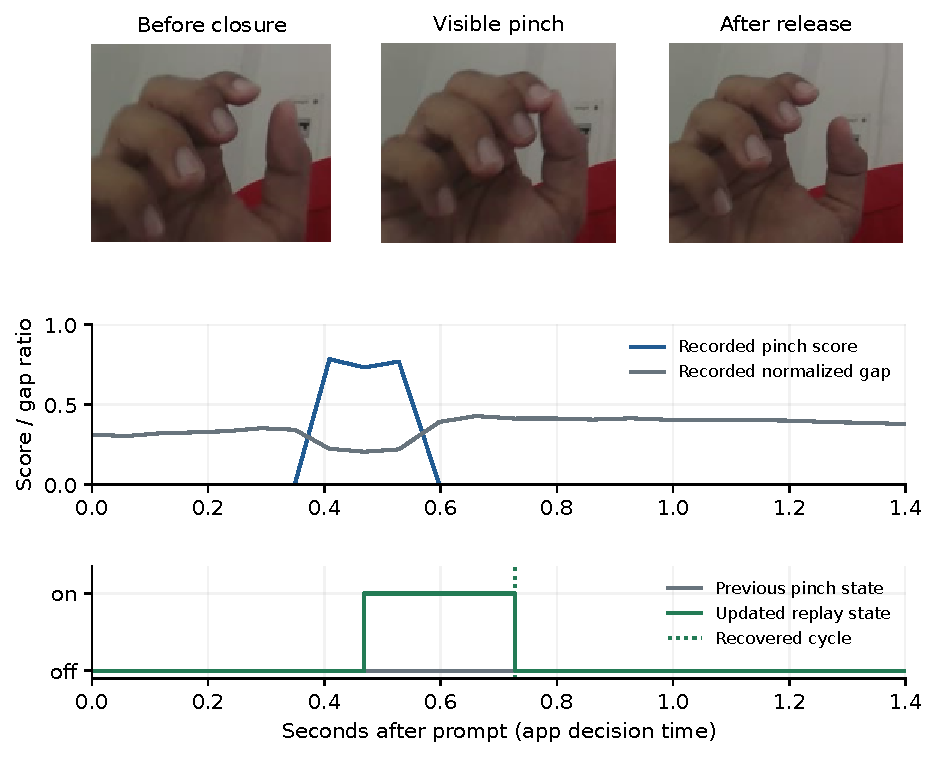
\includegraphics[width=\linewidth]{images/pinch_case.pdf}
\caption{Recorded hand crops and evidence for a missed brief pinch. Replaying the same observations with the updated control rule recovers the cycle. The plots compare the original and updated decisions.}
\label{fig:pinchcase}
\end{figure}



\subsection{Synthetic trajectory experiments}
We generated ideal keyboard paths and added controlled disturbances to test decoding and preprocessing choices. These disturbances follow an assumed noise model. The template baseline normalizes shape by subtracting the centroid and dividing by the RMS radius. It also keeps a separate location channel. The \hyperref[app:reproducibility]{appendix} gives the averaging derivation and points to the full experiment notes.

\begin{figure}[H]
\centering
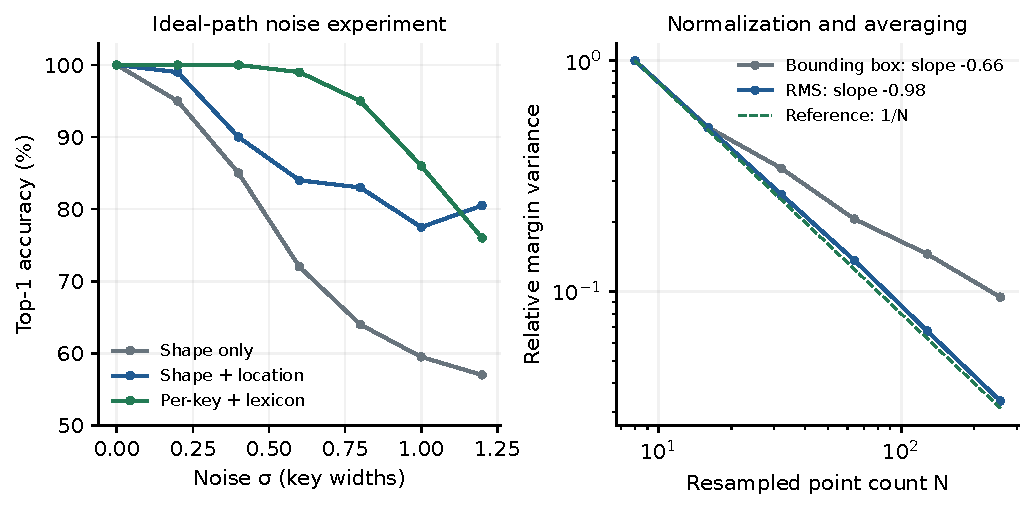
\includegraphics[width=\linewidth]{images/synthetic.pdf}
\caption{Synthetic analyses using generated paths. Left: shape-plus-location and shape-only gesture decoding compared with lexicon-corrected per-key decoding. Right: ranking-margin variance relative to $N=8$, comparing RMS and bounding-box normalization.}
\label{fig:synthetic}
\end{figure}

\textbf{Location is useful alongside shape.} At noise $\sigma=0.4$ key widths, adding location to shape matching raises synthetic top-1 accuracy from 85.0\% to 90.0\%. Under combined disturbances, the same comparison gives 70.4\% versus 82.4\%. We keep both channels in the template baseline. Lexicon-corrected per-key decoding is stronger at the tested noise levels through $\sigma=1.0$. The next tested level is $1.2$, where gesture accuracy is 80.5\% and per-key accuracy is 76.0\%. A finer noise grid would help locate the crossover more precisely.

\textbf{Effect of normalization.} The distance simulation gives perfect accuracy without noise. With fixed image-space noise, accuracy drops from about 99.3\% at 30 cm to 92.7\% at 90 cm. Scaling the coordinates does not make a smaller hand image easier to measure. RMS normalization gives a ranking-variance slope of $-0.977$, close to $1/N$ scaling. Bounding-box normalization gives $-0.664$. This supports using RMS normalization for the template baseline.

\textbf{Preprocessing has diminishing returns.} The smoothing experiment shows the jitter--lag trade-off for the One Euro filter used in the app. Increasing the synthetic path samples beyond roughly 16--32 points has less effect than increasing vocabulary size. Our neural decoder keeps 50 points to match its pretrained features. The type of noise also matters. Shape-plus-location accuracy drops from 94.0\% with independent noise to 82.4\% with combined drift, timing, and speed-dependent disturbances. We therefore test several disturbances and use the separate camera recordings to check tracking and release behavior.

\subsection{Comparison with existing methods and overall discussion}
Table~\ref{tab:comparison} compares the decoders using the same D1 vocabulary, held-out subjects, coordinate degradation, and 50 Hz preprocessing. Other typing studies use different hardware and interaction methods. FineType uses wearable sensors and surface contact, while Shen et al. use headset input \cite{recent03,shen2023}. We use the matched decoder experiment for our numerical comparison.



The two neural models have similar scores on clean D1 input. The difference appears under the webcam and harsh presets, where training on degraded trajectories reduces the accuracy loss. The tracker and pinch detector stay unchanged in this comparison.

In the webcam recordings, missed and split paths were the first problem. Better word ranking became useful once the app captured more complete gestures. The visual pipeline improves capture, while personalization ranks the intended word higher within the captured traces. The total capture gain comes from the combined changes to cropping, state rules, and detector weights.

The lighting update recovers the difficult recorded block and keeps the original 29-attempt results. It slightly lowers the word scores on the older development set. We kept it because the lighting recovery was useful despite that small loss.



\section{Conclusion and future scope}
% Required: resolved issue, method, quantified improvement and two future directions.
WebSwipe converts a pinched hand movement into word suggestions using one webcam. We fine-tuned a pretrained HaGRID gesture detector and personalized a trajectory decoder. MediaPipe tracking stayed frozen. Combining these parts increased complete capture from 8/29 to 23/29 on the original webcam attempts. The final pipeline also recovered 15/15 swipes on replay of the inspected difficult-lighting recording. In the separate nine-subject experiment, degradation training improved simulated-webcam decoder accuracy from 74.6\% to 82.9\%.

The next step is to test the app with new users and measure typing performance. We plan two further studies. The first would collect independent webcam sessions across users, lighting conditions, and viewing angles, with separate training and test sessions. The second would measure typing speed, text errors, latency, and effort in a controlled typing study.

% References replace the unrelated sample bibliography; all borrowed methods and recent works are cited.
\bibliography{mybibfile}
\clearpage
\phantomsection
\section*{Appendix: Reproducibility and audit notes}\label{app:reproducibility}
\newcommand{\suppsection}{\subsection*}
\suppsection{Reproducibility and selected version}
The report covers the app after the 11 October 2026 control update. The detector and decoder weights were trained on 10 October and stayed unchanged during that update. Model weights and full camera recordings are stored separately from the documentation archive.

The model files are \nolinkurl{gesture_lighting_20261010.onnx}, \nolinkurl{gesture_crop_20261010.onnx}, \nolinkurl{decoder_personalized_20261010.pt}, and \nolinkurl{hand_landmarker.task}. The selected settings are detector onset 0.5, continuation 0.3, two onset votes from three observations, 80 ms swipe release, 700 ms standard onset lookback, appearance-confirmed left controls, a 10,000-word lexicon, endpoint weight 1, unigram-prior weight 0, and 50 Hz trajectory preprocessing. The fresh-camera reader is enabled. The left-control implementation is identified by its source hash because its temporal rules cannot be captured by a single threshold.

The app uses NumPy 2.5.3, SciPy 1.18.1, OpenCV-contrib 5.0.0.93, MediaPipe 1.0.1, ONNX Runtime 1.30.0, PyTorch 2.14.0, and wordfreq 3.1.1 with Python 3.13. Full hashes and launch arguments are in \nolinkurl{evidence/runtime_snapshot.json}. The primary detector, reference detector, and decoder hashes begin \texttt{0753c406}, \texttt{b3eb1f95}, and \texttt{3a2dba7d}, respectively. We checked packaging and startup without a camera on Linux for the preceding package. For the latest package, we checked that the source matched and the model files were unchanged. We have not tested the Windows and macOS launchers on those platforms.


\suppsection{Selected left-hand control rules}
For the left hand, the established contact path starts after two observed frames with an appearance score of at least 0.3. An additional fast path accepts a strongly supported closure before the contact median catches up. The closing-motion path needs two consecutive observations with pinch scores of at least 0.7. These must show close fingertips moving together from a recently appearance-confirmed open pose. The gap must be at most 0.27, with a decrease of at least 0.07 in normalized gap within 250 ms. There must be no more than 150 ms between the two observations. Fingers resting close together do not meet the motion requirement.

A fast episode can end after sustained geometric separation or 200 ms of confident visual release. This helps stop a short pinch from becoming an unintended delete. The two release timers run independently. A 200 ms re-entry guard reduces duplicate commands. Holding the pinch for 0.6 seconds triggers deletion.

\suppsection{Investigated variants outside the selected configuration}
The selected demo uses the standard 700 ms evidence-filtered onset buffer. We also tried the experimental \texttt{GuardedStartBuffer} and an online two-component Gaussian-mixture pinch method. Neither is enabled in the selected app. The model still has a fist class from gesture training, but the old fist shortcut is disabled. A held left pinch deletes the word.


\suppsection{Normalization and the limits of noise averaging}
Our SHARK2 comparison uses separate shape and location channels. To normalize shape, we subtract the path's centroid and divide by its RMS radius. A noiseless path keeps the same normalized shape when it is translated or uniformly scaled. The location channel still depends on position. This normalization does not remove perspective changes or preserve the signal-to-noise ratio when the hand appears smaller in the image.

A useful idealized calculation considers fixed templates $T_w$ and independent zero-mean noise $\epsilon_i$ with per-axis variance $\sigma^2$. Without estimating normalization from the noisy observations,
\begin{equation}
D_w=\frac{1}{N}\sum_i\lVert x_i+\epsilon_i-T_{w,i}\rVert^2,
\qquad \mathbb{E}[D_w]=D_w^{\rm clean}+2\sigma^2.
\end{equation}
In this idealized model, every candidate receives the same expected additive term. The variance of an averaged ranking margin can decrease as $1/N$ when the contributions are bounded and independent. Our processing changes those assumptions: smoothing correlates errors, resampling interpolates points, and centering and scale use the same noisy samples. The simulation follows approximately inverse-sample variance with RMS normalization. The exact common offset relies on the idealized assumptions. Per-key input also benefits from lexicon correction and performs better at some tested noise levels.


\suppsection{Supporting records and numerical audit}
The accompanying \href{WebSwipe_LaTeX_Source.zip}{\nolinkurl{WebSwipe_LaTeX_Source.zip}} contains the source, evidence, figure inputs, and build instructions. This appendix is also provided as \href{WebSwipe_Reproducibility_Supplement.pdf}{\nolinkurl{WebSwipe_Reproducibility_Supplement.pdf}}.

The source archive includes diagnostic details in \nolinkurl{evidence/diagnostic_detail_notes.tex}, control checks in \nolinkurl{evidence/control_validation_history.tex}, and synthetic results in \nolinkurl{evidence/synthetic_experiment_notes.tex}. The calculations behind the reported statistics are in \nolinkurl{evidence/review_numerical_audit.json}. The archived control checks include 15 focused software tests for the selected update.

\end{document}
